% Options for packages loaded elsewhere
\PassOptionsToPackage{unicode}{hyperref}
\PassOptionsToPackage{hyphens}{url}
\PassOptionsToPackage{dvipsnames,svgnames,x11names}{xcolor}
%
\documentclass[
  12pt,
  letterpaper,
]{book}

\usepackage{amsmath,amssymb}
\usepackage{iftex}
\ifPDFTeX
  \usepackage[T1]{fontenc}
  \usepackage[utf8]{inputenc}
  \usepackage{textcomp} % provide euro and other symbols
\else % if luatex or xetex
  \usepackage{unicode-math}
  \defaultfontfeatures{Scale=MatchLowercase}
  \defaultfontfeatures[\rmfamily]{Ligatures=TeX,Scale=1}
\fi
\usepackage{lmodern}
\ifPDFTeX\else  
    % xetex/luatex font selection
    \setmainfont[]{Computer Modern}
\fi
% Use upquote if available, for straight quotes in verbatim environments
\IfFileExists{upquote.sty}{\usepackage{upquote}}{}
\IfFileExists{microtype.sty}{% use microtype if available
  \usepackage[]{microtype}
  \UseMicrotypeSet[protrusion]{basicmath} % disable protrusion for tt fonts
}{}
\makeatletter
\@ifundefined{KOMAClassName}{% if non-KOMA class
  \IfFileExists{parskip.sty}{%
    \usepackage{parskip}
  }{% else
    \setlength{\parindent}{0pt}
    \setlength{\parskip}{6pt plus 2pt minus 1pt}}
}{% if KOMA class
  \KOMAoptions{parskip=half}}
\makeatother
\usepackage{xcolor}
\usepackage[margin=1in]{geometry}
\setlength{\emergencystretch}{3em} % prevent overfull lines
\setcounter{secnumdepth}{3}
% Make \paragraph and \subparagraph free-standing
\makeatletter
\ifx\paragraph\undefined\else
  \let\oldparagraph\paragraph
  \renewcommand{\paragraph}{
    \@ifstar
      \xxxParagraphStar
      \xxxParagraphNoStar
  }
  \newcommand{\xxxParagraphStar}[1]{\oldparagraph*{#1}\mbox{}}
  \newcommand{\xxxParagraphNoStar}[1]{\oldparagraph{#1}\mbox{}}
\fi
\ifx\subparagraph\undefined\else
  \let\oldsubparagraph\subparagraph
  \renewcommand{\subparagraph}{
    \@ifstar
      \xxxSubParagraphStar
      \xxxSubParagraphNoStar
  }
  \newcommand{\xxxSubParagraphStar}[1]{\oldsubparagraph*{#1}\mbox{}}
  \newcommand{\xxxSubParagraphNoStar}[1]{\oldsubparagraph{#1}\mbox{}}
\fi
\makeatother

\usepackage{color}
\usepackage{fancyvrb}
\newcommand{\VerbBar}{|}
\newcommand{\VERB}{\Verb[commandchars=\\\{\}]}
\DefineVerbatimEnvironment{Highlighting}{Verbatim}{commandchars=\\\{\}}
% Add ',fontsize=\small' for more characters per line
\newenvironment{Shaded}{}{}
\newcommand{\AlertTok}[1]{\textcolor[rgb]{1.00,0.33,0.33}{\textbf{#1}}}
\newcommand{\AnnotationTok}[1]{\textcolor[rgb]{0.42,0.45,0.49}{#1}}
\newcommand{\AttributeTok}[1]{\textcolor[rgb]{0.84,0.23,0.29}{#1}}
\newcommand{\BaseNTok}[1]{\textcolor[rgb]{0.00,0.36,0.77}{#1}}
\newcommand{\BuiltInTok}[1]{\textcolor[rgb]{0.84,0.23,0.29}{#1}}
\newcommand{\CharTok}[1]{\textcolor[rgb]{0.01,0.18,0.38}{#1}}
\newcommand{\CommentTok}[1]{\textcolor[rgb]{0.42,0.45,0.49}{#1}}
\newcommand{\CommentVarTok}[1]{\textcolor[rgb]{0.42,0.45,0.49}{#1}}
\newcommand{\ConstantTok}[1]{\textcolor[rgb]{0.00,0.36,0.77}{#1}}
\newcommand{\ControlFlowTok}[1]{\textcolor[rgb]{0.84,0.23,0.29}{#1}}
\newcommand{\DataTypeTok}[1]{\textcolor[rgb]{0.84,0.23,0.29}{#1}}
\newcommand{\DecValTok}[1]{\textcolor[rgb]{0.00,0.36,0.77}{#1}}
\newcommand{\DocumentationTok}[1]{\textcolor[rgb]{0.42,0.45,0.49}{#1}}
\newcommand{\ErrorTok}[1]{\textcolor[rgb]{1.00,0.33,0.33}{\underline{#1}}}
\newcommand{\ExtensionTok}[1]{\textcolor[rgb]{0.84,0.23,0.29}{\textbf{#1}}}
\newcommand{\FloatTok}[1]{\textcolor[rgb]{0.00,0.36,0.77}{#1}}
\newcommand{\FunctionTok}[1]{\textcolor[rgb]{0.44,0.26,0.76}{#1}}
\newcommand{\ImportTok}[1]{\textcolor[rgb]{0.01,0.18,0.38}{#1}}
\newcommand{\InformationTok}[1]{\textcolor[rgb]{0.42,0.45,0.49}{#1}}
\newcommand{\KeywordTok}[1]{\textcolor[rgb]{0.84,0.23,0.29}{#1}}
\newcommand{\NormalTok}[1]{\textcolor[rgb]{0.14,0.16,0.18}{#1}}
\newcommand{\OperatorTok}[1]{\textcolor[rgb]{0.14,0.16,0.18}{#1}}
\newcommand{\OtherTok}[1]{\textcolor[rgb]{0.44,0.26,0.76}{#1}}
\newcommand{\PreprocessorTok}[1]{\textcolor[rgb]{0.84,0.23,0.29}{#1}}
\newcommand{\RegionMarkerTok}[1]{\textcolor[rgb]{0.42,0.45,0.49}{#1}}
\newcommand{\SpecialCharTok}[1]{\textcolor[rgb]{0.00,0.36,0.77}{#1}}
\newcommand{\SpecialStringTok}[1]{\textcolor[rgb]{0.01,0.18,0.38}{#1}}
\newcommand{\StringTok}[1]{\textcolor[rgb]{0.01,0.18,0.38}{#1}}
\newcommand{\VariableTok}[1]{\textcolor[rgb]{0.89,0.38,0.04}{#1}}
\newcommand{\VerbatimStringTok}[1]{\textcolor[rgb]{0.01,0.18,0.38}{#1}}
\newcommand{\WarningTok}[1]{\textcolor[rgb]{1.00,0.33,0.33}{#1}}

\providecommand{\tightlist}{%
  \setlength{\itemsep}{0pt}\setlength{\parskip}{0pt}}\usepackage{longtable,booktabs,array}
\usepackage{calc} % for calculating minipage widths
% Correct order of tables after \paragraph or \subparagraph
\usepackage{etoolbox}
\makeatletter
\patchcmd\longtable{\par}{\if@noskipsec\mbox{}\fi\par}{}{}
\makeatother
% Allow footnotes in longtable head/foot
\IfFileExists{footnotehyper.sty}{\usepackage{footnotehyper}}{\usepackage{footnote}}
\makesavenoteenv{longtable}
\usepackage{graphicx}
\makeatletter
\def\maxwidth{\ifdim\Gin@nat@width>\linewidth\linewidth\else\Gin@nat@width\fi}
\def\maxheight{\ifdim\Gin@nat@height>\textheight\textheight\else\Gin@nat@height\fi}
\makeatother
% Scale images if necessary, so that they will not overflow the page
% margins by default, and it is still possible to overwrite the defaults
% using explicit options in \includegraphics[width, height, ...]{}
\setkeys{Gin}{width=\maxwidth,height=\maxheight,keepaspectratio}
% Set default figure placement to htbp
\makeatletter
\def\fps@figure{htbp}
\makeatother

\usepackage{amsmath}
\usepackage{amssymb}
\usepackage{amsthm}
\makeatletter
\@ifpackageloaded{tcolorbox}{}{\usepackage[skins,breakable]{tcolorbox}}
\@ifpackageloaded{fontawesome5}{}{\usepackage{fontawesome5}}
\definecolor{quarto-callout-color}{HTML}{909090}
\definecolor{quarto-callout-note-color}{HTML}{0758E5}
\definecolor{quarto-callout-important-color}{HTML}{CC1914}
\definecolor{quarto-callout-warning-color}{HTML}{EB9113}
\definecolor{quarto-callout-tip-color}{HTML}{00A047}
\definecolor{quarto-callout-caution-color}{HTML}{FC5300}
\definecolor{quarto-callout-color-frame}{HTML}{acacac}
\definecolor{quarto-callout-note-color-frame}{HTML}{4582ec}
\definecolor{quarto-callout-important-color-frame}{HTML}{d9534f}
\definecolor{quarto-callout-warning-color-frame}{HTML}{f0ad4e}
\definecolor{quarto-callout-tip-color-frame}{HTML}{02b875}
\definecolor{quarto-callout-caution-color-frame}{HTML}{fd7e14}
\makeatother
\makeatletter
\@ifpackageloaded{bookmark}{}{\usepackage{bookmark}}
\makeatother
\makeatletter
\@ifpackageloaded{caption}{}{\usepackage{caption}}
\AtBeginDocument{%
\ifdefined\contentsname
  \renewcommand*\contentsname{Table des matières}
\else
  \newcommand\contentsname{Table des matières}
\fi
\ifdefined\listfigurename
  \renewcommand*\listfigurename{Liste des Figures}
\else
  \newcommand\listfigurename{Liste des Figures}
\fi
\ifdefined\listtablename
  \renewcommand*\listtablename{Liste des Tables}
\else
  \newcommand\listtablename{Liste des Tables}
\fi
\ifdefined\figurename
  \renewcommand*\figurename{Figure}
\else
  \newcommand\figurename{Figure}
\fi
\ifdefined\tablename
  \renewcommand*\tablename{Table}
\else
  \newcommand\tablename{Table}
\fi
}
\@ifpackageloaded{float}{}{\usepackage{float}}
\floatstyle{ruled}
\@ifundefined{c@chapter}{\newfloat{codelisting}{h}{lop}}{\newfloat{codelisting}{h}{lop}[chapter]}
\floatname{codelisting}{Listing}
\newcommand*\listoflistings{\listof{codelisting}{Liste des Listings}}
\usepackage{amsthm}
\theoremstyle{remark}
\AtBeginDocument{\renewcommand*{\proofname}{Preuve}}
\newtheorem*{remark}{Remarque}
\newtheorem*{solution}{Solution}
\newtheorem{refremark}{Remarque}[chapter]
\newtheorem{refsolution}{Solution}[chapter]
\makeatother
\makeatletter
\makeatother
\makeatletter
\@ifpackageloaded{caption}{}{\usepackage{caption}}
\@ifpackageloaded{subcaption}{}{\usepackage{subcaption}}
\makeatother

\ifLuaTeX
\usepackage[bidi=basic]{babel}
\else
\usepackage[bidi=default]{babel}
\fi
\babelprovide[main,import]{french}
\ifPDFTeX
\else
\babelfont{rm}[]{Computer Modern}
\fi
% get rid of language-specific shorthands (see #6817):
\let\LanguageShortHands\languageshorthands
\def\languageshorthands#1{}
\ifLuaTeX
  \usepackage{selnolig}  % disable illegal ligatures
\fi
\usepackage[]{biblatex}
\usepackage{bookmark}

\IfFileExists{xurl.sty}{\usepackage{xurl}}{} % add URL line breaks if available
\urlstyle{same} % disable monospaced font for URLs
\hypersetup{
  pdftitle={MAT-2901 : Mathématiques et technologie},
  pdfauthor={Jérôme Soucy},
  pdflang={fr},
  colorlinks=true,
  linkcolor={blue},
  filecolor={Maroon},
  citecolor={Blue},
  urlcolor={blue},
  pdfcreator={LaTeX via pandoc}}


\title{MAT-2901 : Mathématiques et technologie}
\author{Jérôme Soucy}
\date{}

\begin{document}
\frontmatter
\maketitle

\renewcommand*\contentsname{Table des matières}
{
\hypersetup{linkcolor=}
\setcounter{tocdepth}{2}
\tableofcontents
}
\listoffigures
\listoftables

\mainmatter
\bookmarksetup{startatroot}

\chapter*{Présentation}\label{pruxe9sentation}
\addcontentsline{toc}{chapter}{Présentation}

\markboth{Présentation}{Présentation}

Bienvenue sur un site web complémentaire au site monPortail du cours
\textbf{MAT-2904 : Complément d'analyse}, à l'Université Laval.

Ce site contient principalement des séries d'exercices conçues pour
accompagner les étudiants et étudiantes dans le cours. Chaque série
d'exercices est soigneusement élaborée pour approfondir votre
compréhension des concepts clés et vous préparer aux évaluations.

\section*{Les fonctions exponentielles et
logarithmiques}\label{les-fonctions-exponentielles-et-logarithmiques}
\addcontentsline{toc}{section}{Les fonctions exponentielles et
logarithmiques}

\markright{Les fonctions exponentielles et logarithmiques}

Ce document vous invite à explorer en profondeur les fonctions
exponentielles et logarithmiques, des outils mathématiques essentiels
tant en théorie qu'en applications pratiques. À travers onze exercices
soigneusement structurés, vous allez découvrir les multiples facettes de
ces fonctions.

Nous commençons par des exercices techniques de résolution d'équations
exponentielles, avant d'aborder des problèmes plus théoriques qui vous
feront découvrir les propriétés fondamentales de la fonction
exponentielle, notamment son unicité comme solution de l'équation
différentielle f'=f.

Le document intègre également des applications concrètes avec des
problèmes d'intérêts composés et de croissance de populations
bactériennes, illustrant ainsi l'utilité pratique de ces fonctions.

Nous terminons par une exploration rigoureuse de la définition du nombre
e, démontrant comment ce nombre fondamental émerge naturellement des
limites de suites. Les solutions détaillées vous guideront à travers les
raisonnements mathématiques nécessaires pour maîtriser ces concepts clés
de l'analyse mathématique.

\section*{Les fonctions puissances}\label{les-fonctions-puissances}
\addcontentsline{toc}{section}{Les fonctions puissances}

\markright{Les fonctions puissances}

Ce document vous propose une exploration approfondie des fonctions
puissances, un concept fondamental en analyse mathématique. À travers
onze exercices progressifs, vous allez consolider votre compréhension
des propriétés algébriques et analytiques de ces fonctions.

Nous commençons par établir les propriétés fondamentales des puissances
en utilisant la définition \(x^{\alpha} = e^{\alpha \log x}\), puis nous
abordons des questions plus subtiles comme la rationalité des puissances
de nombres irrationnels.

Le document vous guide ensuite vers l'étude des dérivées des fonctions
puissances, avec une attention particulière portée à l'analyse complète
de la fonction racine cubique.

Les exercices culminent avec des applications pratiques :

\begin{itemize}
\tightlist
\item
  Calcul de limites
\item
  Résolution d'équations et d'inéquations
\item
  Calcul d'intégrales faisant intervenir des puissances réelles
\end{itemize}

Chaque exercice est accompagné d'une solution détaillée et, lorsque
pertinent, de représentations graphiques pour faciliter votre
compréhension.

\section*{L'intégrale de Riemann}\label{lintuxe9grale-de-riemann}
\addcontentsline{toc}{section}{L'intégrale de Riemann}

\markright{L'intégrale de Riemann}

Ce document vous propose une série d'exercices approfondis sur
l'intégrale de Riemann, un concept fondamental en analyse mathématique.
Vous y trouverez six questions (incluant plusieurs sous-questions) qui
vous permettront de maîtriser différentes techniques d'intégration et de
comprendre leurs applications.

La première partie vous invite à pratiquer l'intégration indéfinie à
travers douze cas différents, chacun nécessitant des techniques
spécifiques comme :

\begin{itemize}
\tightlist
\item
  Les changements de variables
\item
  L'intégration par parties
\item
  La décomposition en fractions partielles
\end{itemize}

Les exercices suivants vous amènent vers des concepts plus avancés :

\begin{itemize}
\tightlist
\item
  Le calcul d'intégrales définies, y compris avec des bornes infinies
\item
  Le calcul d'aire entre des courbes
\item
  Une démonstration rigoureuse par la méthode de Riemann
\item
  Des questions plus théoriques sur les propriétés des fonctions
  impaires dans l'intégration
\end{itemize}

Chaque exercice est accompagné d'une solution détaillée qui vous permet
de comprendre pas à pas la méthode de résolution.

\section*{Les fonctions
hyperboliques}\label{les-fonctions-hyperboliques}
\addcontentsline{toc}{section}{Les fonctions hyperboliques}

\markright{Les fonctions hyperboliques}

Dans cette série d'exercices sur les fonctions hyperboliques, nous
explorons d'abord les fonctions de base sinh, cosh et tanh, en mettant
l'accent sur leurs graphiques et leurs propriétés fondamentales. Une
attention particulière est portée à la fonction tanh et sa réciproque
arctanh, où nous démontrons notamment la formule importante reliant
arctanh(x) au logarithme naturel. Les graphiques sont systématiquement
tracés pour visualiser le comportement de ces fonctions.

La série progresse ensuite vers des aspects plus théoriques avec la
démonstration d'identités hyperboliques importantes, comme la formule
d'addition pour cosh(x+y). Ces identités sont suivies d'exercices de
résolution d'équations impliquant les fonctions sinh et cosh, montrant
comment ces fonctions sont interconnectées par des relations
fondamentales comme cosh²(x) - sinh²(x) = 1. Une partie intéressante de
la série est consacrée à la comparaison graphique de sinh et cosh, nous
permettant de mieux comprendre leurs comportements respectifs.

La série se termine par une application concrète et fascinante : l'étude
de la chaînette, qui représente la forme que prend un câble suspendu
sous son propre poids. Ce problème pratique nous montre comment les
fonctions hyperboliques apparaissent naturellement dans des situations
physiques réelles, illustrant ainsi leur importance au-delà des
mathématiques pures.

\section*{Licence et attributions}\label{licence-et-attributions}
\addcontentsline{toc}{section}{Licence et attributions}

\markright{Licence et attributions}

Ce site et son contenu sont mis à disposition sous licence Creative
Commons Attribution - Pas d'Utilisation Commerciale (CC BY-NC).

\begin{tcolorbox}[enhanced jigsaw, colbacktitle=quarto-callout-note-color!10!white, leftrule=.75mm, title=\textcolor{quarto-callout-note-color}{\faInfo}\hspace{0.5em}{Droits d'utilisation}, opacityback=0, toptitle=1mm, toprule=.15mm, opacitybacktitle=0.6, colframe=quarto-callout-note-color-frame, breakable, bottomrule=.15mm, rightrule=.15mm, titlerule=0mm, left=2mm, bottomtitle=1mm, arc=.35mm, colback=white, coltitle=black]

Vous êtes libre de :

\begin{itemize}
\tightlist
\item
  Partager, copier et redistribuer le contenu
\item
  Adapter et transformer le contenu
\end{itemize}

À condition de :

\begin{itemize}
\tightlist
\item
  Créditer la source en citant l'auteur du présent document avec un lien
  vers ce site
\item
  Ne pas faire d'usage commercial du contenu
\end{itemize}

Une partie du code présenté sur ce site a été généré avec l'assistance
de l'intelligence artificielle Claude (Anthropic), tout en étant vérifié
et adapté pour garantir son exactitude et sa pertinence pédagogique.

\end{tcolorbox}

\begin{figure}

\begin{minipage}{0.50\linewidth}


\includegraphics[width=2.60417in,height=\textheight]{by-nc.png}

\subcaption{\label{}Licence Creative Commons BY-NC}
\end{minipage}%
%
\begin{minipage}{0.50\linewidth}


\includegraphics[width=0.78125in,height=\textheight]{AIA.jpg}

\subcaption{\label{}Généré avec assistance IA}
\end{minipage}%

\caption{\label{fig-ccIA}Certains éléments de code de ce site ont été
générés par l'IA. Vous êtes libre d'utiliser le contenu de ce site dans
la mesure où vous citez la source et n'en tirez pas de bénéfice
financier.}

\end{figure}%

\part{Théorie}

\chapter{Le ballon météorologique}\label{le-ballon-muxe9tuxe9orologique}

Un ballon est lancé verticalement vers le haut avec une vitesse initiale
de 10 m/s. En tenant compte de la résistance de l'air, sa hauteur (en
mètres) après \(t\) secondes est donnée par la fonction :

\[h(t) = 50\ln(\cosh(0.2t)) + 10t - 4.9t^2\]

À quel moment le ballon atteint-il son altitude maximale ?

\subsection{1. Visualisation du
problème}\label{visualisation-du-probluxe8me}

Commençons par visualiser la hauteur du ballon en fonction du temps :

\begin{Shaded}
\begin{Highlighting}[]
\FunctionTok{library}\NormalTok{(ggplot2)}
\FunctionTok{library}\NormalTok{(dplyr)}

\CommentTok{\# Fonction hauteur}
\NormalTok{h }\OtherTok{\textless{}{-}} \ControlFlowTok{function}\NormalTok{(t) \{}
  \DecValTok{50} \SpecialCharTok{*} \FunctionTok{log}\NormalTok{(}\FunctionTok{cosh}\NormalTok{(}\FloatTok{0.2} \SpecialCharTok{*}\NormalTok{ t)) }\SpecialCharTok{+} \DecValTok{10} \SpecialCharTok{*}\NormalTok{ t }\SpecialCharTok{{-}} \FloatTok{4.9} \SpecialCharTok{*}\NormalTok{ t}\SpecialCharTok{\^{}}\DecValTok{2}
\NormalTok{\}}

\CommentTok{\# Création des données}
\NormalTok{t\_vals }\OtherTok{\textless{}{-}} \FunctionTok{seq}\NormalTok{(}\DecValTok{0}\NormalTok{, }\DecValTok{3}\NormalTok{, }\AttributeTok{by =} \FloatTok{0.01}\NormalTok{)}
\NormalTok{height\_data }\OtherTok{\textless{}{-}} \FunctionTok{data.frame}\NormalTok{(}
  \AttributeTok{t =}\NormalTok{ t\_vals,}
  \AttributeTok{height =} \FunctionTok{sapply}\NormalTok{(t\_vals, h)}
\NormalTok{)}

\CommentTok{\# Graphique}
\FunctionTok{ggplot}\NormalTok{(height\_data, }\FunctionTok{aes}\NormalTok{(}\AttributeTok{x =}\NormalTok{ t, }\AttributeTok{y =}\NormalTok{ height)) }\SpecialCharTok{+}
  \FunctionTok{geom\_line}\NormalTok{(}\AttributeTok{color =} \StringTok{"blue"}\NormalTok{, }\AttributeTok{size =} \DecValTok{1}\NormalTok{) }\SpecialCharTok{+}
  \FunctionTok{labs}\NormalTok{(}\AttributeTok{x =} \StringTok{"Temps (s)"}\NormalTok{, }\AttributeTok{y =} \StringTok{"Hauteur (m)"}\NormalTok{) }\SpecialCharTok{+}
  \FunctionTok{theme\_minimal}\NormalTok{() }\SpecialCharTok{+}
  \FunctionTok{ggtitle}\NormalTok{(}\StringTok{"Trajectoire du ballon"}\NormalTok{)}
\end{Highlighting}
\end{Shaded}

\begin{figure}[H]

\centering{

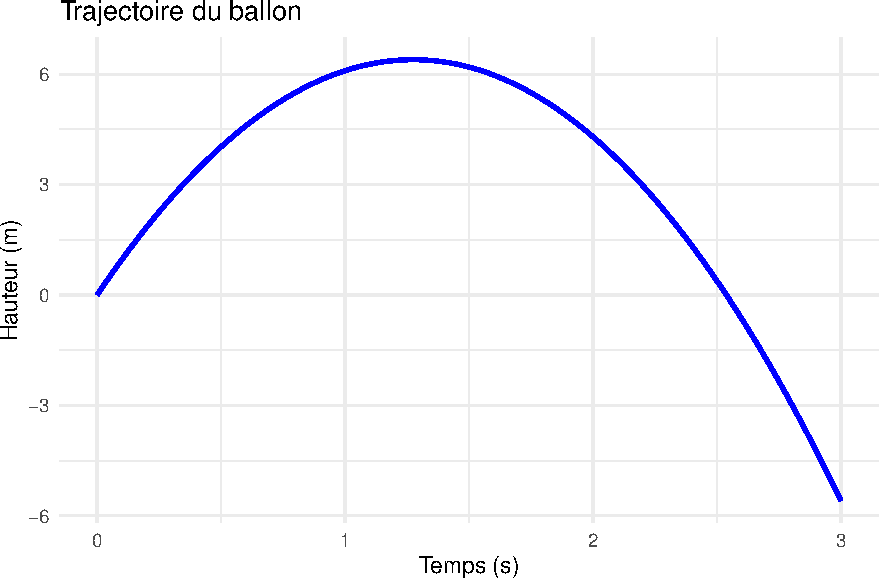
\includegraphics{theorie/TIntroFractales/TIntroFractales_files/figure-pdf/fig-hauteur-1.pdf}

}

\caption{\label{fig-hauteur}Hauteur du ballon en fonction du temps}

\end{figure}%

\subsection{2. La vitesse du ballon}\label{la-vitesse-du-ballon}

La vitesse est la dérivée de la hauteur. Pour trouver le point
culminant, nous devons trouver quand la vitesse est nulle.

\[v(t) = h'(t) = 10\tanh(0.2t) + 10 - 9.8t\]

Visualisons la vitesse :

\begin{Shaded}
\begin{Highlighting}[]
\CommentTok{\# Fonction vitesse}
\NormalTok{v }\OtherTok{\textless{}{-}} \ControlFlowTok{function}\NormalTok{(t) \{}
  \DecValTok{10} \SpecialCharTok{*} \FunctionTok{tanh}\NormalTok{(}\FloatTok{0.2} \SpecialCharTok{*}\NormalTok{ t) }\SpecialCharTok{+} \DecValTok{10} \SpecialCharTok{{-}} \FloatTok{9.8} \SpecialCharTok{*}\NormalTok{ t}
\NormalTok{\}}

\CommentTok{\# Création des données}
\NormalTok{velocity\_data }\OtherTok{\textless{}{-}} \FunctionTok{data.frame}\NormalTok{(}
  \AttributeTok{t =}\NormalTok{ t\_vals,}
  \AttributeTok{velocity =} \FunctionTok{sapply}\NormalTok{(t\_vals, v)}
\NormalTok{)}

\CommentTok{\# Graphique}
\FunctionTok{ggplot}\NormalTok{(velocity\_data, }\FunctionTok{aes}\NormalTok{(}\AttributeTok{x =}\NormalTok{ t, }\AttributeTok{y =}\NormalTok{ velocity)) }\SpecialCharTok{+}
  \FunctionTok{geom\_line}\NormalTok{(}\AttributeTok{color =} \StringTok{"red"}\NormalTok{, }\AttributeTok{size =} \DecValTok{1}\NormalTok{) }\SpecialCharTok{+}
  \FunctionTok{geom\_hline}\NormalTok{(}\AttributeTok{yintercept =} \DecValTok{0}\NormalTok{, }\AttributeTok{linetype =} \StringTok{"dashed"}\NormalTok{) }\SpecialCharTok{+}
  \FunctionTok{labs}\NormalTok{(}\AttributeTok{x =} \StringTok{"Temps (s)"}\NormalTok{, }\AttributeTok{y =} \StringTok{"Vitesse (m/s)"}\NormalTok{) }\SpecialCharTok{+}
  \FunctionTok{theme\_minimal}\NormalTok{() }\SpecialCharTok{+}
  \FunctionTok{ggtitle}\NormalTok{(}\StringTok{"Vitesse du ballon"}\NormalTok{)}
\end{Highlighting}
\end{Shaded}

\begin{figure}[H]

\centering{

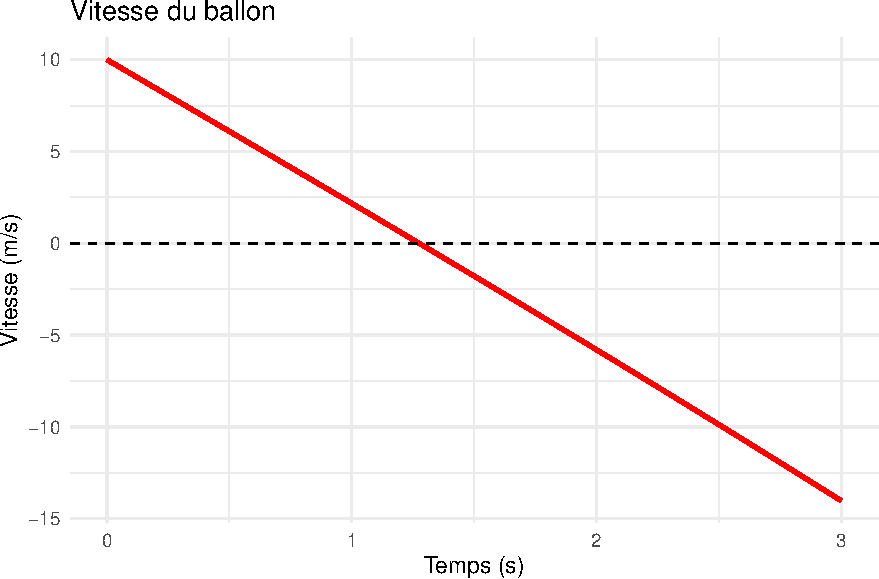
\includegraphics{theorie/TIntroFractales/TIntroFractales_files/figure-pdf/fig-vitesse-1.pdf}

}

\caption{\label{fig-vitesse}Vitesse du ballon en fonction du temps}

\end{figure}%

\subsection{3. Méthode de
Newton-Raphson}\label{muxe9thode-de-newton-raphson}

Pour trouver quand la vitesse est nulle, nous devons résoudre :
\[f(t) = 10\tanh(0.2t) + 10 - 9.8t = 0\]

La dérivée de cette fonction est :
\[f'(t) = 2\,\text{sech}^2(0.2t) - 9.8\]

Implémentons la méthode de Newton-Raphson :

\begin{Shaded}
\begin{Highlighting}[]
\CommentTok{\# Fonction f(t) et sa dérivée}
\NormalTok{f }\OtherTok{\textless{}{-}} \ControlFlowTok{function}\NormalTok{(t) \{}
  \DecValTok{10} \SpecialCharTok{*} \FunctionTok{tanh}\NormalTok{(}\FloatTok{0.2} \SpecialCharTok{*}\NormalTok{ t) }\SpecialCharTok{+} \DecValTok{10} \SpecialCharTok{{-}} \FloatTok{9.8} \SpecialCharTok{*}\NormalTok{ t}
\NormalTok{\}}

\NormalTok{f\_prime }\OtherTok{\textless{}{-}} \ControlFlowTok{function}\NormalTok{(t) \{}
  \DecValTok{2} \SpecialCharTok{*}\NormalTok{ (}\DecValTok{1} \SpecialCharTok{/} \FunctionTok{cosh}\NormalTok{(}\FloatTok{0.2} \SpecialCharTok{*}\NormalTok{ t))}\SpecialCharTok{\^{}}\DecValTok{2} \SpecialCharTok{{-}} \FloatTok{9.8}
\NormalTok{\}}

\CommentTok{\# Fonction Newton{-}Raphson}
\NormalTok{newton\_raphson }\OtherTok{\textless{}{-}} \ControlFlowTok{function}\NormalTok{(x0, }\AttributeTok{tolerance =} \FloatTok{1e{-}6}\NormalTok{, }\AttributeTok{max\_iter =} \DecValTok{100}\NormalTok{) \{}
\NormalTok{  x }\OtherTok{\textless{}{-}}\NormalTok{ x0}
\NormalTok{  iterations }\OtherTok{\textless{}{-}} \FunctionTok{data.frame}\NormalTok{(}
    \AttributeTok{iteration =} \DecValTok{0}\NormalTok{,}
    \AttributeTok{x =}\NormalTok{ x0,}
    \AttributeTok{f\_x =} \FunctionTok{f}\NormalTok{(x0)}
\NormalTok{  )}
  
  \ControlFlowTok{for}\NormalTok{ (i }\ControlFlowTok{in} \DecValTok{1}\SpecialCharTok{:}\NormalTok{max\_iter) \{}
\NormalTok{    x\_new }\OtherTok{\textless{}{-}}\NormalTok{ x }\SpecialCharTok{{-}} \FunctionTok{f}\NormalTok{(x) }\SpecialCharTok{/} \FunctionTok{f\_prime}\NormalTok{(x)}
    
\NormalTok{    iterations }\OtherTok{\textless{}{-}} \FunctionTok{rbind}\NormalTok{(iterations, }
                       \FunctionTok{data.frame}\NormalTok{(}\AttributeTok{iteration =}\NormalTok{ i,}
                                \AttributeTok{x =}\NormalTok{ x\_new,}
                                \AttributeTok{f\_x =} \FunctionTok{f}\NormalTok{(x\_new)))}
    
    \ControlFlowTok{if}\NormalTok{ (}\FunctionTok{abs}\NormalTok{(x\_new }\SpecialCharTok{{-}}\NormalTok{ x) }\SpecialCharTok{\textless{}}\NormalTok{ tolerance) \{}
      \ControlFlowTok{break}
\NormalTok{    \}}
\NormalTok{    x }\OtherTok{\textless{}{-}}\NormalTok{ x\_new}
\NormalTok{  \}}
  
  \FunctionTok{return}\NormalTok{(iterations)}
\NormalTok{\}}

\CommentTok{\# Application avec x0 = 1}
\NormalTok{resultats }\OtherTok{\textless{}{-}} \FunctionTok{newton\_raphson}\NormalTok{(}\DecValTok{1}\NormalTok{)}

\CommentTok{\# Affichage des résultats}
\NormalTok{knitr}\SpecialCharTok{::}\FunctionTok{kable}\NormalTok{(resultats,}
             \AttributeTok{col.names =} \FunctionTok{c}\NormalTok{(}\StringTok{"Itération"}\NormalTok{, }\StringTok{"t (secondes)"}\NormalTok{, }\StringTok{"f(t)"}\NormalTok{),}
             \AttributeTok{digits =} \DecValTok{6}\NormalTok{,}
             \AttributeTok{caption =} \StringTok{"Résultats de la méthode de Newton{-}Raphson"}\NormalTok{)}
\end{Highlighting}
\end{Shaded}

\begin{longtable}[]{@{}rrr@{}}
\caption{Résultats de la méthode de Newton-Raphson}\tabularnewline
\toprule\noalign{}
Itération & t (secondes) & f(t) \\
\midrule\noalign{}
\endfirsthead
\toprule\noalign{}
Itération & t (secondes) & f(t) \\
\midrule\noalign{}
\endhead
\bottomrule\noalign{}
\endlastfoot
0 & 1.000000 & 2.173753 \\
1 & 1.275930 & -0.006241 \\
2 & 1.275143 & 0.000000 \\
3 & 1.275143 & 0.000000 \\
\end{longtable}

\subsection{4. Vérification graphique}\label{vuxe9rification-graphique}

Visualisons la convergence sur le graphique de la vitesse :

\begin{Shaded}
\begin{Highlighting}[]
\CommentTok{\# Filtrer les données pour l\textquotesingle{}intervalle [1, 1.5]}
\NormalTok{velocity\_data\_zoom }\OtherTok{\textless{}{-}}\NormalTok{ velocity\_data }\SpecialCharTok{\%\textgreater{}\%} 
  \FunctionTok{filter}\NormalTok{(t }\SpecialCharTok{\textgreater{}=} \DecValTok{1} \SpecialCharTok{\&}\NormalTok{ t }\SpecialCharTok{\textless{}=} \FloatTok{1.5}\NormalTok{)}

\CommentTok{\# Ajout des points d\textquotesingle{}itération au graphique de vitesse avec zoom}
\FunctionTok{ggplot}\NormalTok{(velocity\_data\_zoom, }\FunctionTok{aes}\NormalTok{(}\AttributeTok{x =}\NormalTok{ t, }\AttributeTok{y =}\NormalTok{ velocity)) }\SpecialCharTok{+}
  \FunctionTok{geom\_line}\NormalTok{(}\AttributeTok{color =} \StringTok{"red"}\NormalTok{, }\AttributeTok{size =} \DecValTok{1}\NormalTok{) }\SpecialCharTok{+}
  \FunctionTok{geom\_hline}\NormalTok{(}\AttributeTok{yintercept =} \DecValTok{0}\NormalTok{, }\AttributeTok{linetype =} \StringTok{"dashed"}\NormalTok{) }\SpecialCharTok{+}
  \FunctionTok{geom\_point}\NormalTok{(}\AttributeTok{data =}\NormalTok{ resultats, }
             \FunctionTok{aes}\NormalTok{(}\AttributeTok{x =}\NormalTok{ x, }\AttributeTok{y =}\NormalTok{ f\_x),}
             \AttributeTok{color =} \StringTok{"blue"}\NormalTok{,}
             \AttributeTok{size =} \DecValTok{3}\NormalTok{) }\SpecialCharTok{+}
  \FunctionTok{geom\_path}\NormalTok{(}\AttributeTok{data =}\NormalTok{ resultats, }
            \FunctionTok{aes}\NormalTok{(}\AttributeTok{x =}\NormalTok{ x, }\AttributeTok{y =}\NormalTok{ f\_x),}
            \AttributeTok{color =} \StringTok{"blue"}\NormalTok{,}
            \AttributeTok{arrow =} \FunctionTok{arrow}\NormalTok{(}\AttributeTok{length =} \FunctionTok{unit}\NormalTok{(}\FloatTok{0.2}\NormalTok{, }\StringTok{"cm"}\NormalTok{)),}
            \AttributeTok{size =} \FloatTok{0.5}\NormalTok{) }\SpecialCharTok{+}
  \FunctionTok{labs}\NormalTok{(}\AttributeTok{x =} \StringTok{"Temps (s)"}\NormalTok{, }\AttributeTok{y =} \StringTok{"Vitesse (m/s)"}\NormalTok{) }\SpecialCharTok{+}
  \FunctionTok{scale\_x\_continuous}\NormalTok{(}\AttributeTok{limits =} \FunctionTok{c}\NormalTok{(}\DecValTok{1}\NormalTok{, }\FloatTok{1.5}\NormalTok{),}
                    \AttributeTok{breaks =} \FunctionTok{seq}\NormalTok{(}\DecValTok{1}\NormalTok{, }\FloatTok{1.5}\NormalTok{, }\FloatTok{0.1}\NormalTok{)) }\SpecialCharTok{+}
  \FunctionTok{theme\_minimal}\NormalTok{() }\SpecialCharTok{+}
  \FunctionTok{ggtitle}\NormalTok{(}\StringTok{"Convergence de la méthode de Newton{-}Raphson (zoom)"}\NormalTok{) }\SpecialCharTok{+}
  \FunctionTok{theme}\NormalTok{(}\AttributeTok{axis.text =} \FunctionTok{element\_text}\NormalTok{(}\AttributeTok{size =} \DecValTok{10}\NormalTok{),}
        \AttributeTok{axis.title =} \FunctionTok{element\_text}\NormalTok{(}\AttributeTok{size =} \DecValTok{12}\NormalTok{))}
\end{Highlighting}
\end{Shaded}

\begin{figure}[H]

\centering{

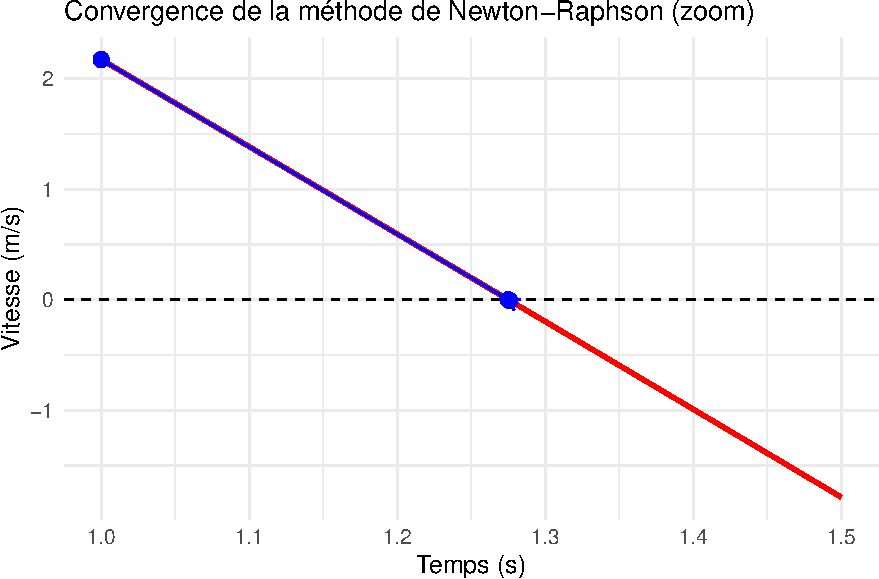
\includegraphics{theorie/TIntroFractales/TIntroFractales_files/figure-pdf/fig-convergence-1.pdf}

}

\caption{\label{fig-convergence}Convergence de la méthode de
Newton-Raphson}

\end{figure}%

\subsection{Conclusion}\label{conclusion}

La méthode de Newton-Raphson converge rapidement vers la solution : le
ballon atteint son altitude maximale après environ 1.275 secondes.

À cet instant, l'altitude du ballon est de 6.39 mètres.

\part{Exercices}

\chapter{Les équations
différentielles}\label{les-uxe9quations-diffuxe9rentielles}

\section{Question 1}\label{question-1}

Résoudre l'équation différentielle : \(\frac{dy}{dx} = 2xy\)

\begin{solution}
D'abord, on réorganise l'équation comme \(\frac{1}{y}dy = 2x dx\). Nous
avons divisé par \(y\), que nous supposons différente de la fonction
identiquement nulle pour la suite. Remarquons que la fonction
identiquement nulle est une solution de l'équation différentielle.

Intégrons les deux membres de l'équation :
\(\int \frac{1}{y}dy = \int 2x dx\). Nous obtenons
que\(\ln|y| = x^2 + C\). En prenant l'exponentielle, nous obtenons que
\(|y|=e^{C}e^{x^2}\). Ainsi, \(|y|=C_1e^{x^2}\), où \(C_1\) est une
constante strictement positive. De là nous avons que \(y=C_2e^{x^2}\),
où \(C_2\) est une constante réelle non nulle. Finalement, on se
rappelle que \(y=0\) est solution de l'équation différentielle de
départ, ce qui nous permet d'écrire que l'ensemble des solutions de
l'équation différentielle est formé de toutes les fonctions de la forme
\(y=Ke^{x^2}, K\in\mathbb{R}\).
\end{solution}

\section{Question 2}\label{question-2}

Résoudre l'équation différentielle \[\frac{dy}{dx} = \frac{x}{y}.\]

\begin{solution}
On sépare les variables pour obtenir l'équation \(y dy = x dx\). On
intègre ensuite les deux membres de l'équation :
\(\int y dy = \int x dx\). Nous obtenons que
\(\frac{y^2}{2} = \frac{x^2}{2} + C\). Ainsi, la solution générale est
\[y = \pm\sqrt{x^2 + K},\] où \(K\) est une constante arbitraire.
\end{solution}

\section{Question 3}\label{question-3}

Résoudre l'équation différentielle \[\frac{dy}{dx} = \frac{y}{x}.\]

\begin{solution}
On sépare les variables pour obtenir l'équation
\(\frac{dy}{y} = \frac{dx}{x}\). On a divisé par \(y\), on supposera
donc pour la suite que \(y\) n'est pas identiquement nulle. On remarque
aussi que la fonction identiquement nulle est une solution de l'équation
différentielle.

On intègre ensuite les deux membres de l'équation :
\(\int \frac{dy}{y} = \int \frac{dx}{x}\). Nous obtenons que
\(\ln|y| = \ln|x| + C\). Comme la fonction \(\ln\) est une bijection des
réels strictement positifs vers \(\mathbb{R}\), il existe un unique
\(k\in\mathbb{R}_{>0}\) tel que \(C=\ln k\). Ainsi,
\[\ln|y| = \ln|x| + C=\ln|x| + \ln k=\ln k|x|.\] L'injectivité de la
fonction \(\ln\) implique que \(y=\pm k|x|\). Si on trace ces courbes,
on constate qu'il s'agit des droites de pente non nulle passant par
l'origine. Comme la droite \(y(x)=0\) est une solution (on l'a remarqué
plus tôt), l'ensemble des solutions consiste à être l'ensemble des
droites passant par l'origine, c'est-à-dire aux courbes d'équation
\(y(x)=Dx, D\in\mathbb{R}\).
\end{solution}

\section{Question 4}\label{question-4}

Résoudre l'équation différentielle : \(\frac{dy}{dx} = y^2\)

\begin{solution}
On constate que \(y(x)=0\) est une solution. Maintenant, pour trouver
les solutions non nulles, divisons par \(y^2\) pour séparer les
variables. On obtient ainsi que \[\frac{dy}{y^2} = dx.\] En intégrant
chacun des membres de l'équation, nous obtenons que
\[-\frac{1}{y} = x + C,\] où \(C\) est une constante réelle arbitraire.
On isole par la suite \(y\), pour obtenir une solution de la forme
\[y = -\frac{1}{x + K},\] où \(K\) est une constante réelle arbitraire.
\end{solution}

\section{Question 5}\label{question-5}

Résoudre l'équation différentielle : \(\frac{dy}{dx} = e^{x-y}\)

\begin{solution}
Pour résoudre cette équation, commençons par réorganiser les termes afin
de séparer les variables. En multipliant chaque membre par \(e^y\), nous
obtenons \[e^y dy = e^x dx.\] En intégrant chacun des membres de
l'équation, nous obtenons que \[e^y = e^x + C,\] où \(C\) est une
constante réelle arbitraire. On isole par la suite \(y\) en appliquant
le logarithme naturel de chaque côté, pour obtenir une solution de la
forme \[y(x) = \ln(e^x + C).\]
\end{solution}

\section{Question 6}\label{question-6}

Lorsqu'une personne avale une substance toxique, son foie tente de
l'éliminer. Généralement, le taux d'élimination de la quantité de
substance encore présente dans l'organisme au temps \(t\) --- que nous
noterons \(Q(t)\) --- est proportionnel à la quantité de substance
encore présente dans l'organisme au temps \(t\). Au temps \(t=0\),
Jocelyn a avalé une quantité \(Q_0\) d'un liquide toxique. Après 3
heures, on a estimé que son foie avait éliminé 50\% du liquide. D'après
ce modèle, combien d'heures se seront écoulées entre le moment où
Jocelyn a avalé le produit et celui où il en aura éliminé 90\%?

\section{Question 7}\label{question-7}

Un vêtement pesant 50 grammes est plongée dans un bassin d'eau. En le
sortant du bassin, au temps \(t=0\), sa masse est de 200 grammes. On
l'étend immédiatement sur une corde à linge pour qu'il sèche. On observe
qu'après 180 minutes, sa masse est de 100 grammes. Combien de minutes se
seront écoulées entre le moment où le vêtement est sorti du bassin et
celui où il aura évacué 99\% de l'eau qu'il contenait initialement?
Arrondissez à la minute. Pour répondre à cette question, on fera
l'hypothèse que le taux d'évaporation d'eau dans le vêtement est
proportionnel à la quantité d'eau présente dans celui-ci.

\section{Question 8}\label{question-8}

Un réservoir contient initialement 100 kg de lait écrémé (le pourcentage
de matière grasse du lait écrémé est de 0 \%). Au temps \(t=0\), on
commence à y verser, à un taux constant de 10 kg/minute, du lait dont le
pourcentage de matière grasse est de 4 \%. Au même moment, un drain
évacue le lait du réservoir vers le camion réfrigérée, à un taux
constant de 10 kg/minute. Pour répondre à cette question, on fera
l'hypothèse que le mélangeur du réservoir permet de garder son contenu
homogène.

\begin{enumerate}
\tightlist
\item
  Soit \(M\) la masse (en kg) de matière grasse dans le réservoir en
  fonction du temps \(t\) (en minutes). Trouvez la fonction \(M(t)\).
\item
  Évaluez \(\lim_{t\rightarrow\infty}M(t)\).
\end{enumerate}

\begin{solution}
\leavevmode

\begin{enumerate}
\item
  Pendant un petit intervalle de temps \(\Delta t\) minutes, il entre
  10\(\Delta t\) kilogrammes de lait, qui contient une proportion 4/100
  de matières grasses. Donc la masse de matières grasses entrant est
  \[M_{\text{entrant}} = \frac{4}{100} \times 10\Delta t = 0{,}4 \Delta t\]

  Pendant le même intervalle, il sort une masse \(10\Delta t\) de lait.
  La proportion de matières grasses dans ce lait est \(M(t)/100\).
  Ainsi, on a
  \[M_{\text{entrant}} = \frac{M(t)}{100} \times 10\Delta t = \frac{M(t)}{10} \Delta t.\]

  Le changement dans \(M(t)\) est donc
  \[\Delta M = M_{\text{entrant}} - M_{\text{sortant}} = 0{,}4 \Delta t - \frac{M(t)}{10} \Delta t.\]
  Ainsi \[\frac{\Delta M}{\Delta t} = 0{,}4 - \frac{M(t)}{10}.\] Quand
  \(\Delta t\) tend vers 0, le membre de gauche tend vers \(M'(t)\), et
  on obtient \[M'(t) = 0{,}4 - \frac{M(t)}{10}.\] Cette équation est
  séparable. On a \[\frac{dM}{0{,}4 - \frac{M}{10}} = dt,\] qui est
  équivalente à \[\int \frac{10dM}{4 - M} = \int dt.\] On intègre et on
  obtient que \[-10 \ln|4 - M| = t + C,\] équation qui est équivalente à
  \[|4 - M| = ke^{-t/10}.\] Puisque \(M(0) = 0\), on en déduit que
  \(k = 4\) et finalement \[M(t) = 4 - 4e^{-t/10}.\]
\item
  Puisque \(e^{-t/10} \to 0\) quand \(t \to \infty\), on a
  \(\lim_{t \to \infty} M(t) = 4\). Intuitivement, ce résultat est
  évident car à la longue, on s'attend à ce que l'état initial devienne
  négligeable et que la proportion de gras dans le lait du réservoir
  soit la même que celle du lait qu'on y ajoute.
\end{enumerate}

\end{solution}


\backmatter
\printbibliography



\end{document}
